\chapter{Specifikacija programske potpore}
		
	\section{Funkcionalni zahtjevi}
			
			\textbf{\textit{dio 1. revizije}}\\
			
			\textit{Navesti \textbf{dionike} koji imaju \textbf{interes u ovom sustavu} ili  \textbf{su nositelji odgovornosti}. To su prije svega korisnici, ali i administratori sustava, naručitelji, razvojni tim.}\\
				
			\textit{Navesti \textbf{aktore} koji izravno \textbf{koriste} ili \textbf{komuniciraju sa sustavom}. Oni mogu imati inicijatorsku ulogu, tj. započinju određene procese u sustavu ili samo sudioničku ulogu, tj. obavljaju određeni posao. Za svakog aktora navesti funkcionalne zahtjeve koji se na njega odnose.}\\
			
			
			\noindent \textbf{Dionici:}
			
			\begin{packed_enum}
				
				\item Sudionik
				\item Animator				
				\item Organizator
				
			\end{packed_enum}
			
			\noindent \textbf{Aktori i njihovi funkcionalni zahtjevi:}
			
			
			\begin{packed_enum}
				\item  \underbar{Neregistrirani/neprijavljeni korisnik (inicijator) može:}
				
				\begin{packed_enum}
					
					\item pregledati osnovne informacije o kampu
					\item prijaviti se na kamp (u kapacitetu sudionika ili animatora)
					\item  registrirati se u sustav pomoću podataka dobivenih mailom
					\item prijaviti se u sustav s korisničkim imenom i lozinkom
				\end{packed_enum}
			
				\item  \underbar{Korisnik (sudionik, organizator, animator)(inicijator) može:}
				
				\begin{packed_enum}
					
					\item pregledavati i mijenjati svoje korisničke podatke
					\item izbrisati svoj korisnički račun 
					
				\end{packed_enum}
					\item  \underbar{Sudionik, animator (inicijator) može:}
				\begin{packed_enum}
					
					\item vidjeti odbrojavanje do početka kampa (prije početka kampa)
					\item kontaktirati organizatora (prije početka kampa)
					\item pregledati svoj raspored aktivnosti
					\item vidjeti popis aktivnosti na kojima je sudjelovao te ih ocijeniti i ostaviti komentar
					\item po završetku kampa ocijeniti i ostaviti komentar za cjelokupno iskustvo
					
				\end{packed_enum}
					\item  \underbar{Sudionik (inicijator) može:}
				\begin{packed_enum}
					
				    \item vidjeti svoju grupu, popis njenih članova, i njihove kontakt podatke, kao i animatora s kojima će raditi/je radio te njihove kontakt podatke
					
				\end{packed_enum}
					\item  \underbar{Animator (inicijator) može:}
				\begin{packed_enum}
					
					\item vidjeti popis svih grupa, njihovih članova i drugih animatora, kao i njihove kontakt podatke
				
				\end{packed_enum}
					\item  \underbar{Baza podataka (sudionik) može:}
				\begin{packed_enum}
					
					\item pohraniti sve podatke o korisnicima, aktivnostima, grupama i ocjenjivanju
					
				\end{packed_enum}
	
		    		\item  \underbar{Organizator (inicijator) može:}
		    	\begin{packed_enum}
		    		
		    		\item vidjeti popis svih registriranih korisnika, aktivnosti, grupa i ocjenjivanja, uređivati te popise i brisati stavke tih popisa
		    		\item uređivati osnovne informacije početne stranice
		    		\item definirati aktivnosti te im pridruživati animatore
		    		\item zadati vrijeme prijava na kamp za sudionike i/ili animatore
		    		\item vidjeti popis prijava, te ih prihvatiti ili odbiti
		    		\item odrediti broj grupa na kampu
		    		\item premjestiti sudionika u drugu grupu
		    		\item  puniti raspored s aktivnostima, uređivati ga i brisati aktivnosti iz njega
		    		
		    	\end{packed_enum}
			
			\end{packed_enum}
			
			\eject 
			
			
				
			\subsection{Obrasci uporabe}
				
				\textbf{\textit{dio 1. revizije}}
				
				\subsubsection{Opis obrazaca uporabe}
					\textit{Funkcionalne zahtjeve razraditi u obliku obrazaca uporabe. Svaki obrazac je potrebno razraditi prema donjem predlošku. Ukoliko u nekom koraku može doći do odstupanja, potrebno je to odstupanje opisati i po mogućnosti ponuditi rješenje kojim bi se tijek obrasca vratio na osnovni tijek.}\\
					
					
					\noindent \underbar{\textbf{UC1 - Pregled informacija o kampu - sudionik, animator}}
					\begin{packed_item}
						
						\item \textbf{Glavni sudionik: } Korisnik
						\item  \textbf{Cilj:} Pregled informacija o kampu
						\item  \textbf{Sudionici:} Neregistrirani korisnik, baza podataka
						\item  \textbf{Preduvjet:} Informacije o kampu postoje u bazi podataka
						\item  \textbf{Opis osnovnog tijeka:}
						
						\item[] \begin{packed_enum}
							
							\item Korisnik otvara naslovnu stranicu
							
						\end{packed_enum}
						
						
					\end{packed_item}
					
					\noindent \underbar{\textbf{UC2 - Prijava na kamp}}
					\begin{packed_item}
						
						\item \textbf{Glavni sudionik: } Korisnik
						\item  \textbf{Cilj:} Prijava sudjelovanja u kampu
						\item  \textbf{Sudionici:} Neregistrirani korisnik, baza podataka, organizator
						\item  \textbf{Preduvjet:} Vrijeme prijava je aktivno
						\item  \textbf{Opis osnovnog tijeka:} 
						
						\item[] \begin{packed_enum}
							
							\item Korisnik odabire opciju "Prijava"
							\item Korisnik ispunjava svoje podatke
							\item Korisnik odabire opciju "Gotovo"
							\item Organizator prihvaća prijavu
							\item Generiranje korisničkog računa
							\item Ažuriranje baze podataka
							
						\end{packed_enum}
						
						\item  \textbf{Opis mogućih odstupanja:}
						
						\item[] \begin{packed_item}
							
							\item[2.a] Korisnik odustaje od prijave
							\item[4.a] Organizator odbija prijavu
							\item[] \begin{packed_enum}
								
								\item[1.] Korisnika se mailom obavještava da je prijava odbijena
							\end{packed_enum}
						\end{packed_item}
					\end{packed_item}
					
					\noindent \underbar{\textbf{UC3 - Registracija u sustav}}
					\begin{packed_item}
						
						\item \textbf{Glavni sudionik: }Korisnik
						\item  \textbf{Cilj:} Registracija u sustav
						\item  \textbf{Sudionici:} Baza podataka
						\item  \textbf{Preduvjet:} Korisnik neregistriran i poslao je svoju prijavu
						\item  \textbf{Opis osnovnog tijeka:}
						
						\item[] \begin{packed_enum}
							
							\item Korisnik prima podatke za registraciju na mail adresu
							\item Korisnik odabire opciju "Registracija"
							\item Korisnik ispunjava podatke za registraciju i bira lozinku
							\item Ažuriranje baze podataka
						\end{packed_enum}
						
						\item  \textbf{Opis mogućih odstupanja:}
							
					\end{packed_item}
				
					\noindent \underbar{\textbf{UC4 - Prijava u sustav}}
					\begin{packed_item}
						
						\item \textbf{Glavni sudionik: } Korisnik
						\item  \textbf{Cilj:} Prijava u sustav
						\item  \textbf{Sudionici:} Baza podataka
						\item  \textbf{Preduvjet:} Korisnik nije prijavljen
						\item  \textbf{Opis osnovnog tijeka:}
						
						\item[] \begin{packed_enum}
							
							\item Korisnik odabire opciju "Prijava u sustav"
							\item Korisnik upisuje korisničko ime i lozinku
							\item Nakon prijave, korisnik je preusmjeren na opciju "Moj Kamp"
						
						\end{packed_enum}
						
						\item  \textbf{Opis mogućih odstupanja:}
						
						\item[] \begin{packed_item}
							
							\item[2.a] Korisnik upisuje neispravno korisničko ime ili lozinku
							\item[] \begin{packed_enum}
								
								\item Obavijesti korisnika da su podatci neispravni
							\end{packed_enum}
						\end{packed_item}
					\end{packed_item}
				
					\noindent \underbar{\textbf{UC5 - Pregled osobnih podataka}}
					\begin{packed_item}
						
						\item \textbf{Glavni sudionik: }Korisnik
						\item  \textbf{Cilj:} Omogućiti korisniku pregled vlastitih osobnih podataka
						\item  \textbf{Sudionici:} Baza podataka
						\item  \textbf{Preduvjet:} Korisnik je prijavljen u sustav
						\item  \textbf{Opis osnovnog tijeka:}
						
						\item[] \begin{packed_enum}
							
							\item Korisnik odabire opciju "Moj profil"
					
						\end{packed_enum}
						
					\end{packed_item}
				
					\noindent \underbar{\textbf{UC6 - Izmjena osobnih podataka}}
					\begin{packed_item}
						
						\item \textbf{Glavni sudionik: }Korisnik
						\item  \textbf{Cilj:} Omogućiti korisniku izmjenu osobnih podataka
						\item  \textbf{Sudionici:} Baza podataka
						\item  \textbf{Preduvjet:} Korisnik je prijavljen u sustav
						\item  \textbf{Opis osnovnog tijeka:}
						
						\item[] \begin{packed_enum}
							
							\item Korisnik bira opciju "Moj profil"
							\item Korisnik bira opciju "Izmjena podataka"
							\item Korisnik mijenja podatke
							\item Korisnik bira opciju "Potvrdi izmjene"
							\item Ažuriranje baze podataka
						\end{packed_enum}
						
						\item  \textbf{Opis mogućih odstupanja:}
						
						\item[] \begin{packed_item}
							
							\item[2.a] Korisnik odustaje od izmjene podataka
							\item[] \begin{packed_enum}
								
								\item Korisnik odabire opciju "Odustani"
							\end{packed_enum}
						\end{packed_item}
					\end{packed_item}
				
					\noindent \underbar{\textbf{UC7 - Brisanje korisničkog računa}}
					\begin{packed_item}
						
						\item \textbf{Glavni sudionik: }Korisnik
						\item  \textbf{Cilj:} Brisanje postojećeg korisničkog računa
						\item  \textbf{Sudionici:} Baza podataka, neregistrirani korisnik
						\item  \textbf{Preduvjet:} Korisnik je prijavljen
						\item  \textbf{Opis osnovnog tijeka:}
						
						\item[] \begin{packed_enum}
							
							\item Korisnik odabire "Moj profil"
							\item Korisnik odabire opciju "Obriši račun"
							\item Korisnik odabire opciju "Potvrdi"
							\item Baza podataka se ažurira
							\item Neregistrirani korisnik se preusmjeruje na naslovnu stranicu
						\end{packed_enum}
						
						\item  \textbf{Opis mogućih odstupanja:}
						
						\item[] \begin{packed_item}
							
							\item[3.a] Korisnik odustane od brisanja računa
							\item[] \begin{packed_enum}
								
								\item Korisnik odabire opciju "Odustani"
								
							\end{packed_enum}
							
						\end{packed_item}
					\end{packed_item}
					
					\noindent \underbar{\textbf{UC8 - Pregled odbrojavanja do početka kampa}}
					\begin{packed_item}
						
						\item \textbf{Glavni sudionik: }Sudionik, animator
						\item  \textbf{Cilj:} Pregled odbrojavanja do početka kampa
						\item  \textbf{Sudionici:} Baza podataka
						\item  \textbf{Preduvjet:} Kamp još nije počeo, korisnik je prijavljen u sustav
						\item  \textbf{Opis osnovnog tijeka:}
						
						\item[] \begin{packed_enum}
							
							\item Nakon prijave u sustav korisnik je preusmjeren na stranicu "Moj kamp"
							\item Na stranici "Moj kamp" se prikazuje vrijeme do početka
						\end{packed_enum}
					\end{packed_item}
				
					\noindent \underbar{\textbf{UC9 - Kontaktiranje organizatora}}
					\begin{packed_item}
						
						\item \textbf{Glavni sudionik: }Sudionik, animator
						\item  \textbf{Cilj:} Stupanje u kontakt s organizatorom
						\item  \textbf{Sudionici:} Baza podataka
						\item  \textbf{Preduvjet:} Kamp još nije počeo, korisnik je prijavljen u sustav
						\item  \textbf{Opis osnovnog tijeka:}
						
						\item[] \begin{packed_enum}
							
							\item Nakon prijave u sustav korisnik je preusmjeren na stranicu "Moj kamp"
							\item Korisnik odabire opciju "Kontaktirajte nas"
							\item Na novoj stranici se prikazuju kontakt podaci organizatora
						\end{packed_enum}
						
					\end{packed_item}
					
					\noindent \underbar{\textbf{UC10 - Pregled rasporeda aktivnosti}}
					\begin{packed_item}
						
						\item \textbf{Glavni sudionik: }Sudionik, animator
						\item  \textbf{Cilj:} Pregledati svoj raspored aktivnosti
						\item  \textbf{Sudionici:} Baza podataka
						\item  \textbf{Preduvjet:} Kamp je počeo, korisnik je prijavljen u sustav
						\item  \textbf{Opis osnovnog tijeka:}
						
						\item[] \begin{packed_enum}
							
							\item Nakon prijave u sustav korisnik je preusmjeren na stranicu "Moj kamp"
							\item Na stranici "Moj kamp" se prikazuje raspored aktivnosti po danima
						\end{packed_enum}
					\end{packed_item}
				
					\noindent \underbar{\textbf{UC11 - Pregled obavljenih aktivnosti}}
					\begin{packed_item}
						
						\item \textbf{Glavni sudionik: }Sudionik, animator
						\item  \textbf{Cilj:} Pregled obavljenih aktivnosti
						\item  \textbf{Sudionici:} Baza podataka
						\item  \textbf{Preduvjet:} Kamp je počeo, korisnik je prijavljen
						\item  \textbf{Opis osnovnog tijeka:}
						
						\item[] \begin{packed_enum}
							
							\item Korisnik odabire opciju "Obavljene aktivnosti"
							\item Korisniku se prikazuju aktivnosti koje je obavio
						\end{packed_enum}
						
						\item  \textbf{Opis mogućih odstupanja:}
						
						\item[] \begin{packed_item}
							
							\item[2.a] Korisnik nije obavio nijednu aktivnost
							\item[] \begin{packed_enum}
								
								\item Korisniku se prikazuje prigodna poruka
							\end{packed_enum}
						\end{packed_item}
					\end{packed_item}
					
					\noindent \underbar{\textbf{UC12 - Ocjenjivanje i komentiranje obavljenih aktivnosti}}
					\begin{packed_item}
						
						\item \textbf{Glavni sudionik: }Sudionik, animator
						\item  \textbf{Cilj:} Omogućiti povratnu informaciju o aktivnostima
						\item  \textbf{Sudionici:} Baza podataka
						\item  \textbf{Preduvjet:} Kamp je počeo, korisnik je prijavljen
						\item  \textbf{Opis osnovnog tijeka:}
						
						\item[] \begin{packed_enum}
							
							\item Korisnik odabire opciju "Obavljene aktivnosti"
							\item Korisniku se prikazuju aktivnosti koje je obavio
							\item Korisnik odabire aktivnost koju želi ocjeniti i komentirati
							\item Korisnik odabire ocjenu i , opcionalno, upisuje komentar
							\item Korisnik odabire opciju "Potvrdi"
							\item Baza podataka se ažurira
						\end{packed_enum}
						
						\item  \textbf{Opis mogućih odstupanja:}
						
						\item[] \begin{packed_item}
							
							\item[2.a] Korisnik nije obavio nijednu aktivnost
							\item[] \begin{packed_enum}
								
								\item Korisniku se prikazuje prigodna poruka
								
							\end{packed_enum}
							\item[4.a] Korisnik je odustao od ocjenjivanja
							\item[] \begin{packed_enum}
								
								\item Korisnik odabire opciju "Odustani"
								
							\end{packed_enum}
							\item[5.a] Korisnik nije odabrao ocjenu
							\item[] \begin{packed_enum}
								
								\item Korisnika se vraća na biranje ocjene i prikazuje se poruka kako je ocjena obavezna za predaju mišljenja
								
							\end{packed_enum}
							
						\end{packed_item}
					\end{packed_item}
				
					\noindent \underbar{\textbf{UC13 - Ocjenjivanje i komentiranje cjelokupnog iskustva}}
					\begin{packed_item}
						
						\item \textbf{Glavni sudionik: } Sudionik, animator
						\item  \textbf{Cilj:} Ocjeniti i komentirati cjeloukupno iskustvo
						\item  \textbf{Sudionici:} Baza podataka
						\item  \textbf{Preduvjet:} Korisnik je prijavljen, završene su sve aktivnosti u kampu
						\item  \textbf{Opis osnovnog tijeka:}
						
						\item[] \begin{packed_enum}
							
							\item Korisnik odabire opciju "Ocjenjivanje kampa"
							\item Prikazuje se tekstno polje i ocjene za odabrati
							\item Korisnik odabire ocijenu, te opcionalno u tekstno polje zapisuje komentar
							\item Korisnik odabire opciju "Potvrdi"
							\item Zatvara se Ocjenjivanje kampa
							\item Baza podataka se ažurira
						\end{packed_enum}
						
						\item  \textbf{Opis mogućih odstupanja:}
						
						\item[] \begin{packed_item}
							
							\item[1.a] Korisnik nije završio sve aktivnosti
							\item[] \begin{packed_enum}
								
								\item Korisniku se prikazuje prigodna poruka
								
							\end{packed_enum}
							\item[3.a] Korisnik je odustao od ocjenjivanja
							\item[] \begin{packed_enum}
								
								\item Korisniku odabire opciju "Odustani"

							\end{packed_enum}
							\item[4.a] Korisnik nije odabrao ocjenu
							\item[] \begin{packed_enum}
								
								\item Korisnika se vraća na biranje ocjene i prikazuje se poruka kako je ocjena obavezna za predaju mišljenja
								
							\end{packed_enum}
						\end{packed_item}
					\end{packed_item}
					
					\noindent \underbar{\textbf{UC14 - Pregled podataka o vlastitoj grupi i animatorima}}
					\begin{packed_item}
						
						\item \textbf{Glavni sudionik: }Sudionik
						\item  \textbf{Cilj:} Pregledati podatke vlastite grupe i animatora
						\item  \textbf{Sudionici:} Baza podataka
						\item  \textbf{Preduvjet:} Sudionik je dio grupe, sudionik je prijavljen
						\item  \textbf{Opis osnovnog tijeka:}
						
						\item[] \begin{packed_enum}
							
							\item Sudionik odabire opciju "Pregled grupe"
							\item Prikazuju se podatci o korisnikovoj grupi i animatorima
							\item Prikazuju se podatci o korisnikovoj grupi i animatorima
						\end{packed_enum}
						
						\item  \textbf{Opis mogućih odstupanja:}
						
						\item[] \begin{packed_item}
							
							\item[2.a] Sudionik nije dio grupe
							\item[] \begin{packed_enum}
								
								\item Sudioniku se prikazuje prigodna poruka
								
							\end{packed_enum}
							
						\end{packed_item}
					\end{packed_item}
				
					\noindent \underbar{\textbf{UC15 - Pregled podataka o svim grupama i njenim članovima}}
					\begin{packed_item}
						
						\item \textbf{Glavni sudionik: }Animator
						\item  \textbf{Cilj:} Pregledati podatke o svim grupama i njihovim članovima
						\item  \textbf{Sudionici:} Baza podataka
						\item  \textbf{Preduvjet:} Animator je prijavljen
						\item  \textbf{Opis osnovnog tijeka:}
						
						\item[] \begin{packed_enum}
							
							\item Animator odabire opciju "Pregled grupa i članova"
							\item Prikazuju se podatci o grupama i njenim članovima
							\item Klikom na gumb "Izlaz" izlazi se iz pregleda
						\end{packed_enum}
						
						\item  \textbf{Opis mogućih odstupanja:}
						
						\item[] \begin{packed_item}
							
							\item[2.a] U sustavu ne postoje prijavljene grupe
							\item[] \begin{packed_enum}
								
								\item Animatoru se prikazuje prigodna poruka
								
							\end{packed_enum}
							\item[2.b] U sustavu ne postoje prijavljeni članovi
							\item[] \begin{packed_enum}
								
								\item Korisniku se prikazuje prigodna poruka
								
							\end{packed_enum}
							
						\end{packed_item}
					\end{packed_item}
				
					\noindent \underbar{\textbf{UC16 - Pregled podataka o svim animatorima}}
					\begin{packed_item}
					
						\item \textbf{Glavni sudionik: }Animator
						\item  \textbf{Cilj:} Pregledati podatke o svim animatorima
						\item  \textbf{Sudionici:} Baza podatka
						\item  \textbf{Preduvjet:} Animator je prijavljen u sustav
						\item  \textbf{Opis osnovnog tijeka:}
					
						\item[] \begin{packed_enum}
							
							\item Animator odabire opciju "Pregled animatora"
							\item Prikazuju se podatci o animatorima
							\item Klikom na gumb "Izlaz" izlazi se iz pregleda
					\end{packed_enum}
					
					\item  \textbf{Opis mogućih odstupanja:}
					
					\item[] \begin{packed_item}
						
						\item[2.a] U sustavu ne postoje prijavljeni animatori
						\item[] \begin{packed_enum}
							
							\item Animatoru se ispisuje prigodna poruka
							
						\end{packed_enum}
						
						\end{packed_item}
					\end{packed_item}
			
					\noindent \underbar{\textbf{UC17 - Pregled registriranih korisnika}}
					\begin{packed_item}
					
						\item \textbf{Glavni sudionik: } Organizator
						\item  \textbf{Cilj:} Pregledati registrirane korisnike
						\item  \textbf{Sudionici:} Baza podataka
						\item  \textbf{Preduvjet:} Organizator je prijavljen u sustav
						\item  \textbf{Opis osnovnog tijeka:}
						
						\item[] \begin{packed_enum}
							
							\item Organizator odabire opciju "Pregled korisnika"
							\item Prikazuju se podatci o registriranim korisnicima
							\item Klikom na gumb "Izlaz" izlazi se iz pregleda
						\end{packed_enum}
						
						\item  \textbf{Opis mogućih odstupanja:}
						
						\item[] \begin{packed_item}
							
							\item[2.a] U sustvu ne postoje registrirani korisnici
							\item[] \begin{packed_enum}
								
								\item Organizatoru se prikazuje prigodna poruka
								
							\end{packed_enum}
				
						\end{packed_item}
					\end{packed_item}
				
					\noindent \underbar{\textbf{UC18 - Uređivanje registriranog korisnika}}
					\begin{packed_item}
						
						\item \textbf{Glavni sudionik: } Organizator
						\item  \textbf{Cilj:} Urediti registriranog korisnika
						\item  \textbf{Sudionici:} Baza podataka
						\item  \textbf{Preduvjet:} Organizator je prijavljen u sustav
						\item  \textbf{Opis osnovnog tijeka :}
						
						\item[] \begin{packed_enum}
							
							\item Organizator odabire opciju "Pregled korisnika"
							\item Prikazuju se podatci o svim registriranim korisnicima
							\item Organizator odabire željeni korisnički račun koji želi izmijeniti
							\item Organizator odabire opciju "Izmjena podataka korisnika"
							\item Organizator se prikazuju informacije korisnika s mogućnosti izmjena
							\item Organizator izmjeni željene podatke
							\item Klikom na gumb "Spremi" izlazi se iz pregleda
							\item Baza podataka se ažurira
						\end{packed_enum}
						
						\item  \textbf{Opis mogućih odstupanja:}
						
						\item[] \begin{packed_item}
							
							\item[2.a] Organizator ne izmjeni ni jedan podatak
							\item[] \begin{packed_enum}
								
								\item Organizatoru se prikaže prigodna poruka s opcijom vraćanja na izmjenu podataka
								
							\end{packed_enum}
							\item[4.b] Organizator ne pritisne tipku "Spremi" pri izlasku
							\item[] \begin{packed_enum}
								
								\item Organizatoru se prikaže prigodna poruka s opcijom spremanja izmjenjenih podataka
								
							\end{packed_enum}
						\end{packed_item}
					\end{packed_item}
					
					\noindent \underbar{\textbf{UC19 - Brisanje registriranog korisnika}}
					\begin{packed_item}
						
						\item \textbf{Glavni sudionik: }Organizator
						\item  \textbf{Cilj:} Brisanje registriranog korisnika i svih njegovih podataka iz baze podataka
						\item  \textbf{Sudionici:} Baza podataka
						\item  \textbf{Preduvjet:} Organizator je prijavljen u sustav, registrirani korisnik postoji u sustavu
						\item  \textbf{Opis osnovnog tijeka:}
						
						\item[] \begin{packed_enum}
							
							\item Organizator odabire opciju "Upravljanje"
							\item Organizator odabire kamp za koji želi obrisati registriranog korisnika
							\item Organizator odabire opciju "Korisnici"
							\item Organizator odabire korisnika kojeg želi obrisati 
							\item Organizator odabire opciju "Obriši"
							\item Organizator odabire opciju "Potvrdi"
							\item Baza podataka se ažurira
						\end{packed_enum}
						
						\item  \textbf{Opis mogućih odstupanja:}
						
						\item[] \begin{packed_item}
							
							\item[3.a] Organizator odustaje od brisanja računa
							\item[] \begin{packed_enum}
								
								\item Sustav obavještava organizatora da korisnik neće biti obrisan
								
							\end{packed_enum}
							
						\end{packed_item}
					\end{packed_item}
					
					\noindent \underbar{\textbf{UC20 - Unos aktivnosti}}
					\begin{packed_item}
						
						\item \textbf{Glavni sudionik: }Organizator
						\item  \textbf{Cilj:} Unos nove aktivnosti u sustav
						\item  \textbf{Sudionici:} Baza podataka
						\item  \textbf{Preduvjet:} Organizator je prijavljen u sustav
						\item  \textbf{Opis osnovnog tijeka:}
						
						\item[] \begin{packed_enum}
							
							\item Organizator odabire opciju "Upravljanje"
							\item Organizator odabire kamp za koji želi unijeti novu aktivnost
							\item Organizator odabire opciju "Aktivnosti"
							\item Organizator odabire opciju "Unos aktivnosti"
							\item Organizator upisuje podatke koji definiraju aktivnost
							\item Organizator odabire opciju "Potvrdi"
							\item Baza podataka se ažurira
						\end{packed_enum}
						
						\item  \textbf{Opis mogućih odstupanja:}
						
						\item[] \begin{packed_item}
							
							\item[3.a] Korisnik odustaje od unosa aktivnosti
							\item[] \begin{packed_enum}
								
								\item Sustav obavještava korisnika da aktivnosti neće biti unesena u sustav
								
							\end{packed_enum}
							
							\item[6.a] Aktivnost koju je organizator unio već postoji u sustavu
							\item[] \begin{packed_enum}
								
							\item Sustav obavještava organizatora da aktivnost već postoji u sustavu
							\item Organizator mijenja podatke ili odustaje od unosa aktivnosti u sustav
							
							\end{packed_enum}
							\item[6.b] Korisnik nije unio sve potrebne podatke za definiciju aktivnosti
							\item[] \begin{packed_enum}
								
								\item Sustav obavještava organizatora o podatcima koje mora unijeti
								\item Organizator unosi podatke ili odustaje od unosa aktivnosti u sustav
								
							\end{packed_enum}
						
							
						\end{packed_item}
					\end{packed_item}
					
					\noindent \underbar{\textbf{UC21 - Pregled aktivnosti}}
					\begin{packed_item}
						
						\item \textbf{Glavni sudionik: }Organizator
						\item  \textbf{Cilj:} Pregled aktivnosti u sustavu
						\item  \textbf{Sudionici:} Baza podataka
						\item  \textbf{Preduvjet:} Organizator je prijavljen u sustav, aktivnosti postoje u sustavu
						\item  \textbf{Opis osnovnog tijeka:}
						
						\item[] \begin{packed_enum}
							
							\item Organizator odabire opciju "Upravljanje"
							\item Organizator odabire kamp za koji želi pregledati aktivnosti
							\item Organizator odabire opciju "Aktivnosti"
							\item Sustav prikazuje aktivnosti
						\end{packed_enum}
						
						
					\end{packed_item}
				
					\noindent \underbar{\textbf{UC22 - Uređivanje aktivnosti}}
					\begin{packed_item}
						
						\item \textbf{Glavni sudionik: }Organizator
						\item  \textbf{Cilj:} Uređivanje aktivnosti u sustavu
						\item  \textbf{Sudionici:} Baza podataka
						\item  \textbf{Preduvjet:} Organizator je prijavljen u sustav, aktivnosti postoje u sustavu
						\item  \textbf{Opis osnovnog tijeka:}
						
						\item[] \begin{packed_enum}
							
							
							\item Organizator odabire opciju "Upravljanje"
							\item Organizator odabire kamp za koji želi urediti aktivnost
							\item Organizator odabire opciju "Aktivnosti"
							\item Organizator odabire aktivnost koju želi urediti
							\item Organizator mijenja podatke odabrane aktivnosti
							\item Organizator odabire opciju "Potvrdi"
							\item Baza podataka se ažurira
						\end{packed_enum}
						
						\item  \textbf{Opis mogućih odstupanja:}
						
						\item[] \begin{packed_item}
							
							\item[3.a] Organizator odustaje od uređivanja aktivnosti
							\item[] \begin{packed_enum}
								
								\item Sustav obavještava organizatora da promjene na aktivnosti neće biti unesene u sustav
								
							\end{packed_enum}
							
							\item[6.a] Aktivnost koju je organizator unio već postoji u sustavu
							\item[] \begin{packed_enum}
								
								\item Sustav obavještava organizatora da aktivnost već postoji u sustavu
								\item Organizator mijenja podatke ili odustaje od uređivanja aktivnosti 
								
							\end{packed_enum}
							\item[6.b] Organizator nije unio sve potrebne podatke za definiciju aktivnosti
							\item[] \begin{packed_enum}
								
								\item Sustav obavještava organizatora o podatcima koje mora unijeti
								\item Organizator unosi podatke ili odustaje od uređivanja aktivnosti 
								
							\end{packed_enum}
							
						\end{packed_item}
					\end{packed_item}
				
					\noindent \underbar{\textbf{UC23 - Brisanje aktivnosti}}
					\begin{packed_item}
						
						\item \textbf{Glavni sudionik: }Organizator
						\item  \textbf{Cilj:} Brisanje aktivnosti u sustavu
						\item  \textbf{Sudionici:} Baza podataka
						\item  \textbf{Preduvjet:} Organizator je prijavljen u sustav, aktivnosti postoje u sustavu
						\item  \textbf{Opis osnovnog tijeka:}
						
						\item[] \begin{packed_enum}
							
							\item Organizator odabire opciju "Upravljanje"
							\item Organizator odabire kamp za koji želi obrisati aktivnost
							\item Organizator odabire opciju "Aktivnosti"
							\item Organizator odabire aktivnost koju želi obrisati
							\item Organizator odabire opciju "Obriši"
							\item Organizator odabire opciju "Potvrdi"
							\item Baza podataka se ažurira
						\end{packed_enum}
						
						\item  \textbf{Opis mogućih odstupanja:}
						
						\item[] \begin{packed_item}
							
							\item[3.a] Korisnik odustaje od brisanja aktivnosti
							\item[] \begin{packed_enum}
								
								\item Sustav obavještava organizatora da aktivnost neće biti obrisana	
								
							\end{packed_enum}
							
							
						\end{packed_item}
					\end{packed_item}
					
					\noindent \underbar{\textbf{UC24 - Unos grupa}}
					\begin{packed_item}
						
						\item \textbf{Glavni sudionik: }Organizator
						\item  \textbf{Cilj:} Unos grupa u sustav
						\item  \textbf{Sudionici:} Baza podataka
						\item  \textbf{Preduvjet:} Organizator je prijavljen u sustav
						\item  \textbf{Opis osnovnog tijeka:}
						
						\item[] \begin{packed_enum}
							
							
							\item Organizator odabire opciju "Upravljanje"
							\item Organizator odabire kamp za koji želi unijeti grupu
							\item Organizator odabire opciju "Grupe"
							\item Organizator odabire opciju "Unos grupa"
							\item Organizator upisuje broj grupa koje želi stvoriti
							\item Organizator odabire opciju "Potvrdi"
							\item Baza podataka se ažurira
						\end{packed_enum}
						
						\item  \textbf{Opis mogućih odstupanja:}
						
						\item[] \begin{packed_item}
							
							\item[4.a] Organizator odustaje od unosa grupa
							\item[] \begin{packed_enum}
								
								\item Sustav obavještava organizatora da grupe neće biti unesene u sustav
								
							\end{packed_enum}
							
							
						\end{packed_item}
					\end{packed_item}
					
					\noindent \underbar{\textbf{UC25 - Pregled grupa}}
					\begin{packed_item}
						
						\item \textbf{Glavni sudionik: }Organizator
						\item  \textbf{Cilj:} Pregled trenutno upisanih grupa
						\item  \textbf{Sudionici:} Baza podataka
						\item  \textbf{Preduvjet:} Organizator je prijavljen u sustav
						\item  \textbf{Opis osnovnog tijeka:}
						
						\item[] \begin{packed_enum}
							
							\item Organizator odabire opciju "Upravljanje"
							\item Organizator odabire opciju "Grupe"
							\item Organizator odabire opciju "Pregled grupa"
							\item Organizator upisuje željene kriterije pregleda
							\item Organizator pregledava grupe po željenim kriterijima
						\end{packed_enum}
						
						\item  \textbf{Opis mogućih odstupanja:}
						
						\item[] \begin{packed_item}
							
							\item[2.a] Ne postoji niti jedna grupa u bazi podataka
							\item[] \begin{packed_enum}
								
								\item Sustav obavještava organizatora da ne postoje grupe
								\item Organizator odustaje od pregleda grupe
								
							\end{packed_enum}						
						\end{packed_item}
					\end{packed_item}
				
					\noindent \underbar{\textbf{UC26 - Uređivanje grupe}}
					\begin{packed_item}
						
						\item \textbf{Glavni sudionik: } Organizator
						\item  \textbf{Cilj:} Ažuriranje ili upisivanje podataka o grupi
						\item  \textbf{Sudionici:} Baza podataka
						\item  \textbf{Preduvjet:} Organizator je prijavljen u sustav, grupe postoje u sustavu
						\item  \textbf{Opis osnovnog tijeka:}
						
						\item[] \begin{packed_enum}
							
							\item Organizator odabire opciju "Upravljanje"
							\item Organizator odabire opciju "Grupe"
							\item Organizator odabire grupu koju želi urediti
							\item Organizator odabire opciju "Uredi"
							\item Organizator upiše željene podatke
							\item Organizator odabire opciju "Potvrdi"
							\item Baza podataka se ažurira
						\end{packed_enum}
						
						\item  \textbf{Opis mogućih odstupanja:}
						
						\item[] \begin{packed_item}
							
							\item[5.a] Organizator upisuje nedopuštene podatke
							\item[] \begin{packed_enum}
								
								\item Organizatoru se šalje upozorenje o neispravnim podacima
								
							\end{packed_enum}
							\item[5.b] Organizator odustaje od izmjena
							\item [] \begin{packed_enum}
								
								\item Sustav obavještava organizatora da promjene neće biti unesene u sustav
							\end{packed_enum}
						\end{packed_item}
					\end{packed_item}
				
					\noindent \underbar{\textbf{UC27 - Brisanje grupe}}
					\begin{packed_item}
						
						\item \textbf{Glavni sudionik: }Organizator
						\item  \textbf{Cilj:} Brisanje grupe iz baze podataka
						\item  \textbf{Sudionici:} Baza podataka
						\item  \textbf{Preduvjet:} Organizator je prijavljen u sustav
						\item  \textbf{Opis osnovnog tijeka:}
						
						\item[] \begin{packed_enum}
							
							\item Organizator odabire opciju "Upravljanje"
							\item Organizator odabire opciju "Grupe"
							\item Organizator odabire grupu koju želi izbrisati
							\item Organizator odabire opciju "Izbriši grupu"
							\item Baza podataka se ažurira
						\end{packed_enum}
						
						\item  \textbf{Opis mogućih odstupanja:}
						
						\item[] \begin{packed_item}	
							\item[3.a] Organizator odustaje od brisanja grupe
							\item[] \begin{packed_enum}
								
								\item Organizator odabire opciju "Odustani"
								
							\end{packed_enum}

						\end{packed_item}
						
					\end{packed_item}
				
					\noindent \underbar{\textbf{UC28 - Pregled ocjenjivanja}}
					\begin{packed_item}
						
						\item \textbf{Glavni sudionik: }Organizator
						\item  \textbf{Cilj:} Pregled ocjena vezane uz pojedine aktivnosti
						\item  \textbf{Sudionici:} Baza podataka
						\item  \textbf{Preduvjet:} Organizator je prijavljen u sustav, barem jedna aktivnost je ocijenjena
						\item  \textbf{Opis osnovnog tijeka:}
						
						\item[] \begin{packed_enum}
							
							\item Organizator odabire opciju "Objavljene aktivnosti"
							\item Organizator odabire željenu aktivnost
							\item Prikazuju ocjene pripadne aktivnosti

						\end{packed_enum}
						
						\item  \textbf{Opis mogućih odstupanja:}
						
						\item[] \begin{packed_item}
							
							\item[2.a] Odabrana aktivnost još nije ocijenjena
							\item[] \begin{packed_enum}
								
								\item Sustav organizatoru javlja nedostatak ocjene
								
							\end{packed_enum}
							
						\end{packed_item}
					\end{packed_item}										
				
					\noindent \underbar{\textbf{UC29 - Uređivanje ocjenjivanja}}
					\begin{packed_item}
						
						\item \textbf{Glavni sudionik: } Organizator						\item  \textbf{Cilj:} Prepravljanje već unesene ocjene
						\item  \textbf{Sudionici:} Baza podatak
						\item  \textbf{Preduvjet:} Organizator je prijavljen u sustav, korisnik je ocijenio bar jednu aktivnost
						\item  \textbf{Opis osnovnog tijeka:}
						
						\item[] \begin{packed_enum}
							
							\item Organizator odabire opciju "Obavljene aktivnosti"
							\item Organizator odabire željenu aktivnost
							\item Organizator odabire opciju "Uredi ocjenu"
							\item Organizator prepravlja ocjenu
							\item Baza podataka se ažurira
						\end{packed_enum}
						

					\end{packed_item}
					
					\noindent \underbar{\textbf{UC30 - Brisanje ocjenjivanja}}
					\begin{packed_item}
						
						\item \textbf{Glavni sudionik: } Organizator
						\item  \textbf{Cilj:} Brisanje već unesene ocjene
						\item  \textbf{Sudionici:}Baza podataka
						\item  \textbf{Preduvjet:}Organizator je prijavljen u sustav, korisnik je ocijenio bar jednu aktivnost
						\item  \textbf{Opis osnovnog tijeka:}
						
						\item[] \begin{packed_enum}
							
							\item Organizator odabire opciju "Obavljene aktivnosti"
							\item Organizator odabire željenu aktivnost
							\item Organizator odabire opciju "Izbriši ocjenu"
							\item Organizator briše ocjenu
							\item Baza podataka se ažurira
						\end{packed_enum}
						
					\end{packed_item}
					
					\noindent \underbar{\textbf{UC31 - Stvaranje kampa i unos informacija o kampu}}
					\begin{packed_item}
						
						\item \textbf{Glavni sudionik: } Organizator
						\item  \textbf{Cilj:} Stvoriti kamp i unijeti informacije o održavanju kampa
						\item  \textbf{Sudionici:} Baza podataka
						\item  \textbf{Preduvjet:} -
						\item  \textbf{Opis osnovnog tijeka:}
						
						\item[] \begin{packed_enum}
							
							\item Organizator odabire opciju "Upravljanje"
							\item Organizator odabire opciju "Stvori novi kamp"
							\item Organizator upisuje podatke o kampu
							\item Organizator odabire opciju "Unesi"
							\item Baza podataka se ažurira
						\end{packed_enum}
						
						\item  \textbf{Opis mogućih odstupanja:}
						
						\item[] \begin{packed_item}
							\item[3.a] Organizator izlazi iz opcije "Stvori novi kamp"
							\item[] \begin{packed_enum}
								
								\item Sustav obavještava organizatora da se novi kamp neće stvoriti
								
							\end{packed_enum}
							
							\item[4.a] Kamp s takvim podacima već postoji
							\item[] \begin{packed_enum}
								
								\item Sustav obavještava organizatora o već postojećem kampu s istim podacima
								\item Organizator mijenja potrebne podatke
								
							\end{packed_enum}
						\end{packed_item}
					\end{packed_item}
					
					\noindent \underbar{\textbf{UC32 - Pregled informacija o kampu - organizator}}
					\begin{packed_item}
						
						\item \textbf{Glavni sudionik: } Organizator
						\item  \textbf{Cilj:} Pregledati informacije o kampu
						\item  \textbf{Sudionici:} Baza podataka
						\item  \textbf{Preduvjet:} Kamp postoji u sustavu
						\item  \textbf{Opis osnovnog tijeka:}
						
						\item[] \begin{packed_enum}
							
							\item Organizator odabire opciju "Upravljanje"	
							\item Organizator odabire kamp
							\item Aplikacija prikazuje informacije o kampu
						\end{packed_enum}

					\end{packed_item}
					
					\noindent \underbar{\textbf{UC33 - Uređivanje informacija o kampu}}
					\begin{packed_item}
						
						\item \textbf{Glavni sudionik: } Organizator
						\item  \textbf{Cilj:} Urediti informacije o kampu
						\item  \textbf{Sudionici:} Baza podataka
						\item  \textbf{Preduvjet:} Kamp postoji u sustavu
						\item  \textbf{Opis osnovnog tijeka:}
						
						\item[] \begin{packed_enum}
								
							\item Organizator odabire opciju "Upravljanje"
							\item Organizator odabire kamp
							\item Organizator odabire opciju "Uredi"
							\item Organizator mijenja podatke kampa
							\item Organizator odabire opciju "Spremi promjene"
							\item Baza podataka se ažurira
						\end{packed_enum}
						
						\item  \textbf{Opis mogućih odstupanja:}
						
						\item[] \begin{packed_item}
							
							\item[5.a] Organizator promijeni podatke, ali izađe iz opcije "Uredi"
							\item[] \begin{packed_enum}
								
								\item Sustav obavještava organizatora da nije spremio promjene
								
							\end{packed_enum}
	
							
						\end{packed_item}
					\end{packed_item}
				
					\noindent \underbar{\textbf{UC34 - Brisanje kampa}}
					\begin{packed_item}
						
						\item \textbf{Glavni sudionik: } Organizator
						\item  \textbf{Cilj:} Urediti informacije o kampu
						\item  \textbf{Sudionici:} Baza podataka
						\item  \textbf{Preduvjet:} Kamp postoji u sustavu
						\item  \textbf{Opis osnovnog tijeka:}
						
						\item[] \begin{packed_enum}
							
							\item Organizator odabire opciju "Upravljanje"
							\item Organizator odabire kamp
							\item Organizator odabire opciju "Obriši"
							\item Organizator odabire opciju "Potvrdi"
							\item Baza podataka se ažurira
						\end{packed_enum}
						
						\item  \textbf{Opis mogućih odstupanja:}
						
						\item[] \begin{packed_item}
							
							\item[3.a] Organizator odustane od brisanja kampa
							\item[] \begin{packed_enum}
								
								\item Sustav obavještava organizatora da kamp neće biti obrisan
								
							\end{packed_enum}
							
							
						\end{packed_item}
					
					\end{packed_item}
				
				
					\noindent \underbar{\textbf{UC35 - Pregled prijava}}
					\begin{packed_item}
						
						\item \textbf{Glavni sudionik: } Organizator
						\item  \textbf{Cilj:} Pregledati prijave za kamp
						\item  \textbf{Sudionici:} Baza podataka
						\item  \textbf{Preduvjet:} Kamp postoji u sustavu
						\item  \textbf{Opis osnovnog tijeka:}
						
						\item[] \begin{packed_enum}
							\item Organizator odabire opciju "Upravljanje"
							\item Organizator odabire kamp za koji želi pregledati prijave
							\item Organizator odabire opciju "Prijave"
							\item Aplikacija prikazuje prijave 
						\end{packed_enum}								
					\end{packed_item}
				
					\noindent \underbar{\textbf{UC36 - Prihvaćanje ili odbijanje prijave}}
					\begin{packed_item}
						
						\item \textbf{Glavni sudionik: } Organizator
						\item  \textbf{Cilj:} Prihvatiti ili odbiti prijavu za kamp
						\item  \textbf{Sudionici:} Baza podataka
						\item  \textbf{Preduvjet:} Prijava postoji u sustavu
						\item  \textbf{Opis osnovnog tijeka:}
						
						\item[] \begin{packed_enum}
							
							\item Organizator odabire opciju "Upravljanje"
							\item Organizator odabire kamp za koji želi pregledati prijave
							\item Organizator odabire opciju "Prijave"
							\item Organizator bira prijavu
							\item Organizator prihvaća ili odbija prijavu
							\item Organizator odabire opciju "Potvrdi odluku"
							\item Baza podataka se ažurira
							\item Korisniku čija je prijava prihvaćena ili odbijena se šalje odgovarajuća e-mail obavijest
						\end{packed_enum}
						
						\item  \textbf{Opis mogućih odstupanja:}
						
						\item[] \begin{packed_item}
							
							\item[5.a] Organizator odustane od prihvaćanja ili odbijanja prijave
							\item[] \begin{packed_enum}
								
								\item Sustav obavještava organizatora da prijava nije obrađena
								
							\end{packed_enum}												
						\end{packed_item}
					\end{packed_item}
				
					\noindent \underbar{\textbf{UC37 - Dodavanje aktivnosti u raspored}}
					\begin{packed_item}
						
						\item \textbf{Glavni sudionik: } Organizator
						\item  \textbf{Cilj:} Dodati aktivnost u raspored
						\item  \textbf{Sudionici:} Baza podataka, grupa, animatori
						\item  \textbf{Preduvjet:} Aktivnosti, grupe i animatori postoje u sustavu
						\item  \textbf{Opis osnovnog tijeka:}
						
						\item[] \begin{packed_enum}
							
							\item Organizator odabire opciju "Upravljanje"
							\item Organizator odabire kamp za koji želi dodati aktivnost u raspored
							\item Organizator odabire opciju "Raspored"
							\item Organizator odabire opciju "Dodaj aktivnost"
							\item Organizator odabire aktivnost i pridružuje joj grupe i animatore
							\item Organizator odabire opciju "Dodaj"
							\item Baza se ažurira
						\end{packed_enum}
						
						\item  \textbf{Opis mogućih odstupanja:}
						
						\item[] \begin{packed_item}
							
							\item[5.a] Neki od uvjeta dodavanja aktivnosti u raspored je prekršen
							\item[] \begin{packed_enum}
								
								\item Sustav obavještava organizatora o uvjetima koji nisu ispunjeni
								\item Korisnik mijenja potrebne podatke ili odustaje od 
								dodavanja aktivnosti u raspored
								
							\end{packed_enum}			
						\end{packed_item}
					\end{packed_item}
				
					\noindent \underbar{\textbf{UC38 - Uređivanje aktivnosti u rasporedu}}
					\begin{packed_item}
						
						\item \textbf{Glavni sudionik: } Organizator
						\item  \textbf{Cilj:} Urediti aktivnost u rasporedu
						\item  \textbf{Sudionici:} Baza podataka, grupa, animator
						\item  \textbf{Preduvjet:} Aktivnosti, grupe i animatori postoje u sustavu te aktivnost postoji u rasporedu
						\item  \textbf{Opis osnovnog tijeka:}
						
						\item[] \begin{packed_enum}
							
							\item Organizator odabire opciju "Upravljanje"
							\item Organizator odabire kamp za koji želi urediti aktivnost u rasporedu
							\item Organizator odabire opciju "Raspored"
							\item Organizator odabire aktivnost koju želi urediti
							\item Organizator mijenja podatke
							\item Organizator odabire opciju "Spremi promjene"
							\item Baza se ažurira

						\end{packed_enum}
						
						\item  \textbf{Opis mogućih odstupanja:}
						
						\item[] \begin{packed_item}
							
							\item[5.a] Organizator odustane od izmjene podataka
							\item[] \begin{packed_enum}
								
								\item Sustav obavještava organizatora da podaci neće biti izmijenjeni
								
							\end{packed_enum}					
						\end{packed_item}
					\end{packed_item}
				
					\noindent \underbar{\textbf{UC39 - Brisanje aktivnosti rasporeda}}
					\begin{packed_item}

						\item \textbf{Glavni sudionik: } Organizator
						\item  \textbf{Cilj:} Obrisati aktivnost u rasporedu
						\item  \textbf{Sudionici:} Baza podataka
						\item  \textbf{Preduvjet:} Aktivnosti postoji u rasporedu	
						\item  \textbf{Opis osnovnog tijeka:}
						
						\item[] \begin{packed_enum}
							
							\item Organizator odabire opciju "Upravljanje"
							\item Organizator odabire kamp za koji želi obrisati aktivnost u rasporedu
							\item Organizator odabire opciju "Raspored"
							\item Organizator odabire aktivnost koju želi obrisati
							\item Organizator odabire opciju "Obriši"
							\item Organizator odabire opciju "Potvrdi"
							\item Baza se ažurira
		
						\end{packed_enum}
						
						\item  \textbf{Opis mogućih odstupanja:}
						
						\item[] \begin{packed_item}
							
							\item[2.a] Organizator odustane od brisanja aktivnosti
							\item[] \begin{packed_enum}
								
								\item Sustav obavještava organizatora da aktivnost neće biti obrisana

							\end{packed_enum}			
						\end{packed_item}
					\end{packed_item}
				
					\noindent \underbar{\textbf{UC40 - Brisanje rasporeda}}
					\begin{packed_item}
						
						\item \textbf{Glavni sudionik: } Organizator
						\item  \textbf{Cilj:} Obrisati raspored
						\item  \textbf{Sudionici:} Baza podataka
						\item  \textbf{Preduvjet:} Postoje aktivnosti u rasporedu	
						\item  \textbf{Opis osnovnog tijeka:}
						\item[] \begin{packed_enum}
							
							\item Organizator odabire opciju "Upravljanje"
							\item Organizator odabire kamp za koji želi obrisati raspored
							\item Organizator odabire opciju "Raspored"
							\item Organizator odabire opciju "Obriši raspored"
							\item Organizator odabire opciju "Potvrdi"
							\item Baza se ažurira
						\end{packed_enum}
						
						\item  \textbf{Opis mogućih odstupanja:}
						
						\item[] \begin{packed_item}
							
							\item[2.a] Organizator odustane od brisanja rasporeda
							\item[] \begin{packed_enum}
								
								\item Sustav obavještava organizatora da raspored neće biti obrisana

							\end{packed_enum}
						\end{packed_item}
					\end{packed_item}
			\eject	
							
			\subsubsection{Dijagrami obrazaca uporabe}
				
				\begin{figure}[H]
				\centerline{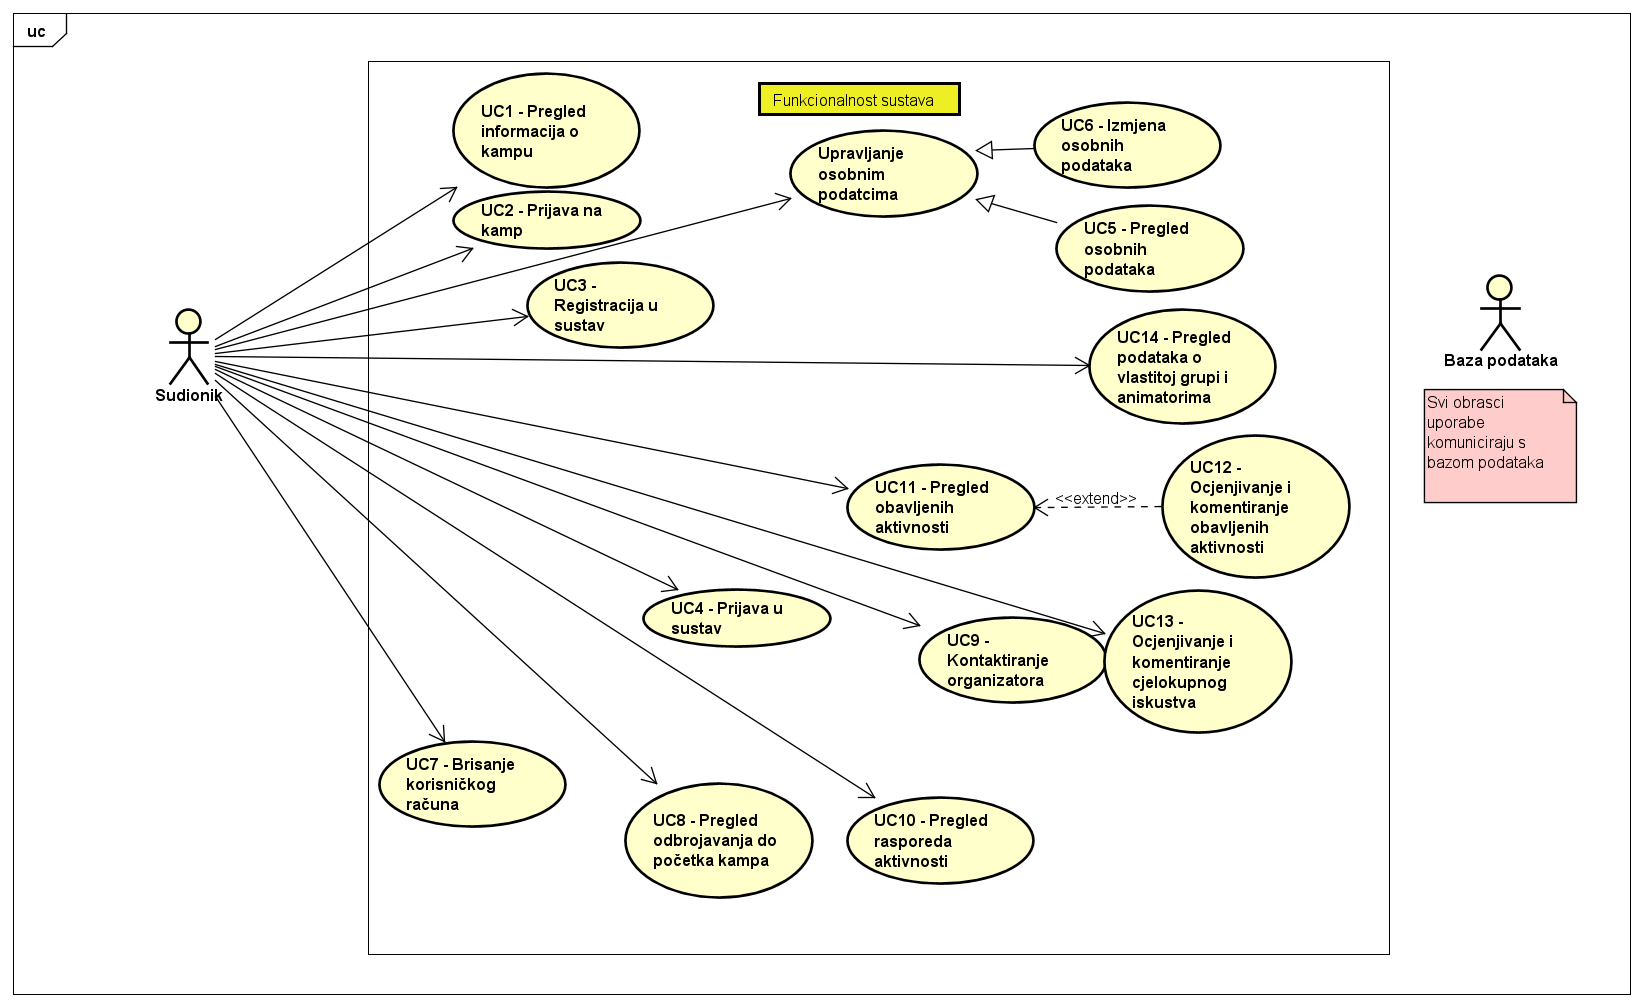
\includegraphics[width=\textwidth]{slike/UC_sudionik.png}}
				\caption{Dijagram obrasca uporabe, funkcionalnosti sudionika}
				\label{fig:ucSudionik}
				\end{figure}
			
				\begin{figure}[H]
					\centerline{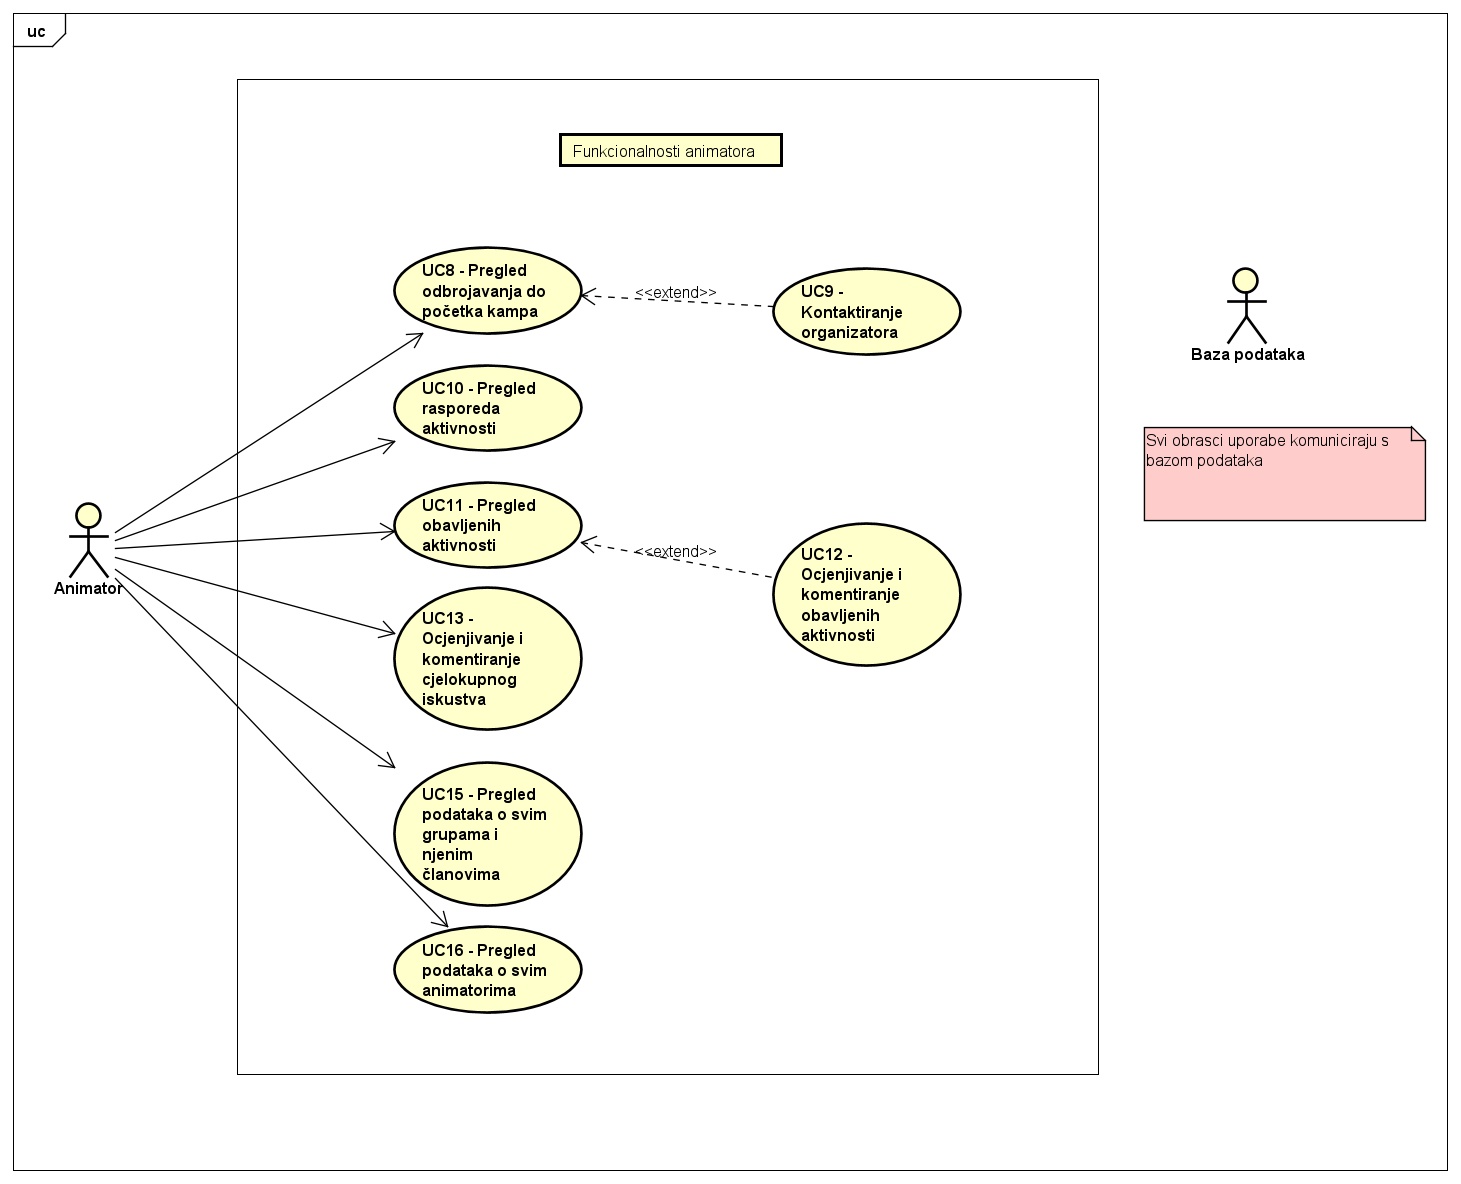
\includegraphics[width=\textwidth]{slike/UC_animator.png}}
					\caption{Dijagram obrasca uporabe, funkcionalnosti animatora}
					\label{fig:ucAnimator}
				\end{figure}
		
				\begin{figure}[H]
					\centerline{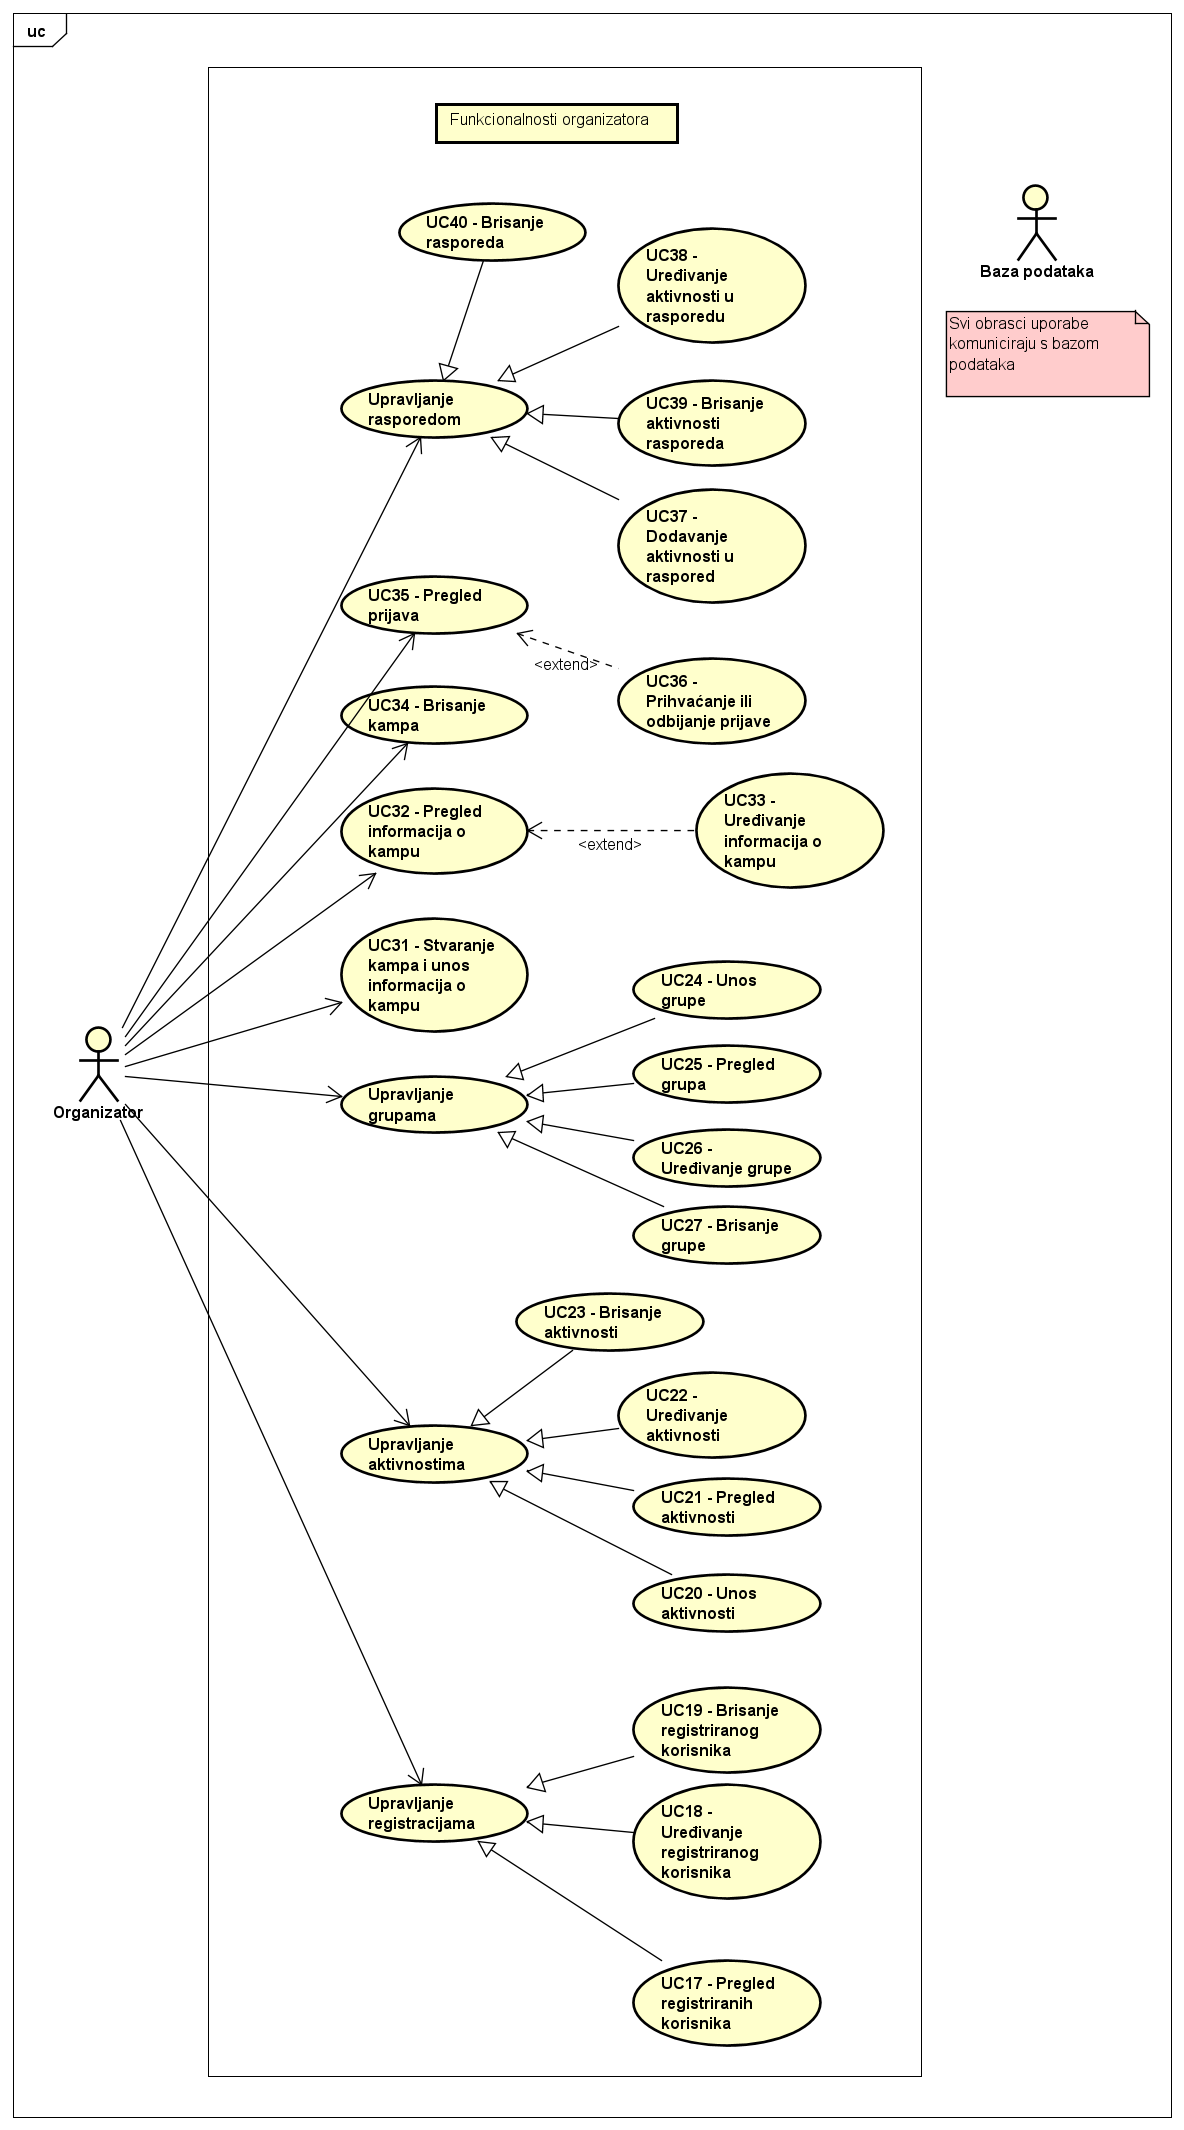
\includegraphics[width=\textwidth, height=0.9\textheight]{slike/UC_organizator.png}}
					\caption{Dijagram obrasca uporabe, funkcionalnosti organizatora}
					\label{fig:ucOrganizator}
				\end{figure}
			
			
			\eject		
				
			\subsection{Sekvencijski dijagrami}

				\textbf{Obrazac uporabe UC4 - Prijava u sustav}

				\noindent Korisnik odabire opciju "Prijava u sustav" i upisuje svoje korisničko ime i lozinku u za to predviđena polja, zatim odabire opciju "U redu". Sustav provjerava postoji li ta kombinacija korisničkog imena i lozinke u bazi podataka. Ako postoji, korisnik se prijavljuje u sustav i nastavlja na stranicu "Moj Kamp". Ako ne postoji, sustav vraća grešku i korisnik ostaje na istoj stranici.
						
				\begin{figure}[H]
					\centerline{\includegraphics[width=\linewidth]{slike/Sekvencijski_dijagram_UC4.png}}
					\caption{Sekvencijski dijagram za UC4}
					\label{fig:sekvencijskiUC4}
				\end{figure}
				\eject
				
				\noindent\textbf{Obrazac uporabe UC36 - Prihvaćanje ili odbijanje prijave}
					
				\noindent Organizator nakon odabira opcije "Upravljanje" odabire opciju "Prijave".Poslužitelj dohvaća popis prijava iz baze podataka i ukoliko prijave postoje, prikazuje ih organizatoru. Organizator filtrira prijave kako bi vidio neobrađene, aktivne prijave. Poslužitelj dohvaća filtrirane prijave iz baze podataka i ukoliko takve prijave postoje, prikazuje ih organizatoru.Organizator odabire prijavu i obrađuje ju, prihvaća ju ili odbija. Nakon što organizator potvrdi svoju odluku, poslužitelj bazi podataka šalje ažurirane podatke. Korisniku čija je prijava obrađena šalje se e-mail obavijest sa statusom njegove prijave i daljnjim uputama.
				\begin{figure}[H]
					\centerline{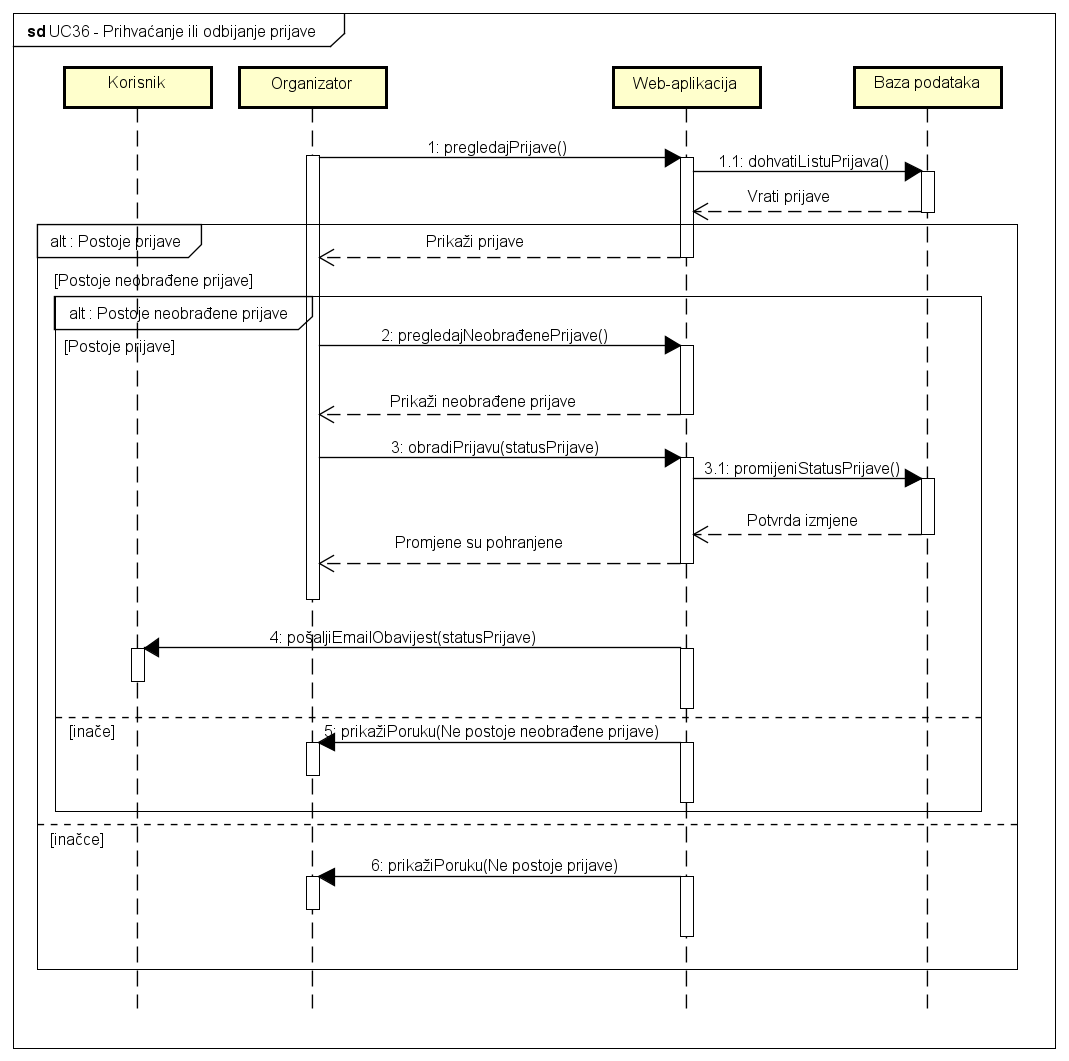
\includegraphics[width=\linewidth]{slike/Sekvencijski_dijagram_UC36.png}}
					\caption{Sekvencijski dijagram za UC36}
					\label{fig:sekvencijskiUC36}
				\end{figure}
				\eject
				
			
			
				
				
	
		\section{Ostali zahtjevi}
			 
			 \begin{packed_item}
			 \item Sustav treba biti implementiran kao web aplikacija koristeći objektno-orijentiranu paradigmu
			 \item Sustav treba omogućiti rad više korisnika u stvarnom vremenu
			 \item Korisničko sučelje i sustav moraju podržavati hrvatsku abecedu (dijakritičke znakove) pri unosu i prikazu tekstualnog sadržaja
			 \item  Neispravno korištenje korisničkog sučelja ne smije narušiti funkcionalnost i rad sustava
			 \item Izvršavanje dijela programa u kojem se pristupa bazi podataka ne smije trajati duže od nekoliko sekundi
			 \item Sustav treba biti jednostavan za korištenje, korisnici se moraju znati koristiti sučeljem bez opširnih uputa
			 \item Nadogradnja sustava ne smije narušavati postojeće funkcionalnosti sustava
			\end{packed_item}
		\eject